\chapter{The Pricing Problem}
\label{sec:the-pricing-problem}

The \textit{Elementary Shortest Path Problem with Resource Constraints} (ESPPRC)
appears as the pricing sub-problem in column generation schemes
for vehicle routing problems, as previously discussed in \cref{sec:branch-and-price}.
As a result, comprehending it is crucial for developing efficient branch-and-price frameworks.
For a literature review on the importance and methodologies
for solving the pricing problem,
we refer the reader to  \cref{sec:solving-the-pricing-problem}.

While the ESPPRC can be studied independently,
we are primarily interested in it in this work from the perspective of pricing for the VRP.
The ESPPRC requests the shortest path (or route)
between a starting and destination vertex on a directed weighted network,
subject to additional resource constraints.
The standard version of the ESPPRC allows for the definition of multiple resources with different semantics, such as time, capacity, gasoline, and more.
The resources are typically monotonically increasing quantities
that increase as the route passes through new edges or vertices \parencite{irnich2005, irnich2007resource}.
Resource consumption can be bounded at various levels of scope,
such as global scope, vertex scope, or arc scope.

The \textit{Elementary Shortest Path Problem with Capacity Constraints} (ESPPCC)
is a subset of the ESPPRC characterized by a single resource: the number of goods.
A global-scoped threshold $Q \in \R_{+}$, the vehicle capacity,
limits the number of goods served during a route.
The ESPPCC can be used to model the pricing sub-problem in the column
generation schemes for the Capacitated Vehicle Routing Problem (CVRP).

We will concentrate on the ESPPCC pricing sub-problem in this work.
However,
it is crucial to acknowledge that the more general ESPPRC is required to model more complex scenarios,
such as the pricing sub-problem induced by the Vehicle Routing Problem with Time Windows (VRPTW).

The \textit{Capacitated Profitable Tour Problem} (CPTP)
is a combinatorial optimization problem that, like the ESPPCC,
can effectively model the CVRP pricing sub-problem.
The CPTP asks for a minimum cost circuit subject to capacity constraints
and can be regarded as a specific case of ESPPCC where the starting
and destination vertices coincide.

\medskip

In \cref{sec:the-elementary-shortest-path-problem-with-capacity-constraints}
we will formally introduce, discuss, and provide an IP formulation for the ESPPCC.
Similarly, in \cref{sec:the-capacitated-profitable-tour-problem},
we will introduce the CPTP and provide an IP formulation and extra valid inequalities.
We will study the basic version of these two problems,
which means that we will not consider non-robust inequalities
that can change the structure of these problems.
However, before delving into the discussion of these two problems,
we will first devote the following section \labelcref{sec:bac-approaches-for-the-pricing-problem}
to a review of the few previous contributions regarding
the use of branch-and-cut approaches for pricing.

\section{Literature Review on Branch-and-Cut approaches applied to the Pricing Problem}
\label{sec:bac-approaches-for-the-pricing-problem}

Label-correcting dynamic programming approaches
dominate as the primary approach to solve the (E)SPPRC in the context of pricing,
see \cite{desrochers1992, feillet2004, righini2004, righini2006, boland2006, righini2008, pugliese2010, baldacci2011, lozano2013, lozano2016, sadykov2021bucket}.
For a more complete discussion, see \cref{sec:solving-the-pricing-problem}.

To our knowledge, branch-and-cut approaches for tackling the (E)SPPRC have received little attention.
The few branch-and-cut contributions that we are aware of are:
(i) \textcite{jepsen2008branchandcut} for the ESPPCC,
(ii) \textcite{jepsen2011,jepsen2014} to the CPTP,
(iii) \textcite{taccari2016, drexl2014} for the related non-resource constrained ESPP
and (iv) \textcite{horvath2016} for the non-elementary RCSP.

To the best of our knowledge,
no branch-and-cut contributions exist for the general ESPPRC version in the literature.
This situation is most likely due to the inherent challenges
of modeling resource constraints with non-global bounds,
such as time window constraints \parencite{jepsen2008branchandcut}.
First, non-global resource bounds necessitate the usage
of directed network-based IP models,
which are twice as large as an undirected equivalent solution.
Second, non-globally bounded resource constraints
can only be modeled as big-M constraints,
which are known to be inherently computationally unstable \parencite{jepsen2008branchandcut}.

\medskip

\textcite{jepsen2008branchandcut} provide an IP mathematical model
for the ESPPCC over an undirected network, along with additional valid inequalities.
In their work, they empirically evaluate the effectiveness of their
branch-and-cut framework in the context of pricing for the CVRP.

\textcite{jepsen2014} investigates the CPTP problem in the context of pricing for the CVRP.
Their work stems from the initial efforts of \textcite{jepsen2008branchandcut}.
\citeauthor{jepsen2014} provide a first tutorial/survey/framework and foundational theory
for further development of the CPTP as a standalone problem or in the context of pricing.
In addition to discussing valid inequalities and their efficient separation,
they propose a model and a branch-and-cut algorithm for solving the CPTP.

\textcite{jepsen2014} conduct a computational study
to assess the competitiveness of their approach
and the usefulness of the employed cutting planes.
Their findings showed that the CPTP-based branch-and-cut framework
was not competitive in solving the CVRP's PP.
Overall, the dynamic programming algorithm appeared to perform vastly better.
Nonetheless, their findings revealed that the branch-and-cut algorithm
solved some larger problem instances in which the labeling algorithm failed to provide a solution.
More specifically, their results showed that:
\begin{enumerate}
	\setlength{\itemsep}{0pt}
	\setlength{\parskip}{0pt}

	\item \label{itm:cptp-branch-and-cut-better-p1}
	      The branch-and-cut (BAC) algorithm appeared to solve some standalone CPTP instances characterized by $800$ customers.
	      Whereas the labeling algorithm ran out of available computation time when solving instances characterized by more than $200$ customers.
	\item \label{itm:cptp-branch-and-cut-better-p2} When the weights of the associated
	      ESPPCC/CPTP network were highly negative,
	      the branch-and-cut algorithm outperformed the labeling algorithm significantly.
	\item \label{itm:cptp-branch-and-cut-better-p3} When the optimal objective value
	      of the problem was very close to the zero threshold,
	      the branch-and-cut framework performed worse.
\end{enumerate}
\Cref{itm:cptp-branch-and-cut-better-p1} relates to standalone CPTP instances and may thus be irrelevant in the pricing context.
With regard to pricing, \cref{itm:cptp-branch-and-cut-better-p2} is of little interest because highly negative weights networks are usually solved through heuristics anyway.
\Cref{itm:cptp-branch-and-cut-better-p3} is probably due to the fact that labeling algorithms are usually optimized to cut off extensive portions of the solution space when the optimal value resides very close to the zero threshold.

Despite their contribution needs to be revisited in light of recent advances on both sides, their findings demonstrated that a branch-and-cut approach could supplement the dynamic programming algorithm for pricing.

\section{The Elementary Shortest Path Problem with Capacity Constraints}
\label{sec:the-elementary-shortest-path-problem-with-capacity-constraints}

This section will go over the \textit{Elementary Shortest Path Problem with Capacity Constraints} (ESPPCC)
in the context of pricing for the CVRP.
We've already seen the general ESPPRC case of this problem in
\cref{sec:column-generation-and-pricing-problem,sec:solving-the-pricing-problem}
but we've never provided a formal description of the mathematical model.
In this section, we consider the basic version of the ESPPCC,
not considering non-robust inequalities at the RMP level.
When non-robust inequalities are used, ESPPCC is insufficient for modeling the pricing problem.
To ensure the correctness of the column generation approach,
a slight variation of the ESPPCC with additional constraints is required.

The ESPPCC asks for the determination of the shortest path on a weighted network
between two vertices $s, t$
subject to a single global resource restriction characterized
by the number of goods available for serving $Q \in \R_{+}$.
The elementarity condition in the ESPPCC problem requires that
no optimal path pass through the same vertices two or more times.
In general, the ESPPCC's underlying network may contain negative cost cycles.
The presence of negative cost cycles makes solving such a problem NP-hard \parencite{dror1994}.
A dynamic programming algorithm
to tackle the elementary version of the problem
was proposed in \textcite{feillet2004}.
In the context of pricing, however, the problem has traditionally been resolved through an SPPRC.
Unlike its elementarity version, the SPPRC can be solved in pseudo-polynomial time
using a much faster dynamic programming algorithm, see \textcite{desrochers1992}.
Unfortunately, relaxing the elementarity condition
slows down column generation and worsens dual bounds,
as discussed previously in \cref{sec:solving-the-pricing-problem}.

\medskip

If the weighted network of the ESPPCC contains no negative-cost cycles, we can safely ignore the elementarity restriction without affecting correctness \parencite{beasley1989}.
A sufficient but not-necessary condition is when the reduced costs are all positive: $\bar{c}_{ij} \ge 0 \quad \forall i, j \in V_0 \cup \Set*{s, t}$.
In this case, an optimal solution to the associated non-elementary SPPRC is an optimal solution to the original elementary version of the problem \parencite{beasley1989}.
The associated SPPRC can then be solved trivially in pseudo-polynomial time.
Initial contributions for tackling the ESPPCC exploited such property.
The resource consumptions were relaxed through a Lagrangian method.
They obtained feasible dual solutions over strictly positive weighted networks using a branch-and-bound scheme and an off-the-shelf standard shortest path algorithm, such as Dijkstra \parencite{sniedovich2006dijkstra}.
To name a few, see the contributions of \textcite{beasley1989, dumitrescu2003improved, carlyle2008, muhandiramge2009simultaneous}.

However, as noted in \textcite{righini2004}, Lagrangian relaxation is only effective when the dualized variables are positive for a significant portion of the Lagrange multipliers search space, limiting the effectiveness of these approaches in the context of pricing.

\subsection{Integer Programming Formulation}
\label{sec:espprc-integer-programming-formulation}

While \textcite{jepsen2008branchandcut} provides
an \textbf{undirected} symmetric network-based formulation for the ESPPCC,
in our presentation, we chose to re-adjust the more-general
\textbf{directed} symmetric network-based ESPPRC formulation
provided in the works of \textcite{beasley1989, toth2002, toth2014}.
As a result, we must readjust/extend the mathematical notation
provided for the undirected CVRP in \cref{sec:cvrp-mathematical-notation}.

\medskip

The ESPPCC is defined over a directed symmetric network
$G^\prime = \Tuple*{V^\prime, A^\prime}$,
where $V^\prime = V_0 \cup \Set*{s, t}$ denotes the set of vertices and $A^\prime$ the set of arcs.
The vertex set $V^\prime$ has size $|V^\prime| = N^\prime = N_0 + 2$, where $N_0$ represents the total customers in the original CVRP problem.
The vertices $s = 0,\ t = N^\prime - 1$ denote respectively the source and sink versions of the depot node.
The arc set $A^\prime$ can be expressed as:
\begin{equation}
	\begin{aligned}
		A^\prime = \  & \Set*{\Tuple*{i, j} \mid i, j \in V_0,\ i \ne j} \\
		              & \cup \Set*{\Tuple*{s, i} \mid i \in V_0}         \\
		              & \cup \Set*{\Tuple*{i, t} \mid i \in V_0}.
	\end{aligned}
\end{equation}
The arc set $A^\prime$ has size $|A^\prime| = N^\prime(N^\prime - 1) + 2(N^\prime - 1)$.
Following the CVRP,
we associate a resource consumption or vertex demand,
to each node of the network: $q_i \quad \forall i \in V^\prime$.
The resource consumption semantics associated with each customer
$i \in V_0$ remains unaltered  from the CVRP, while for the source and sink vertices
we respectively fix $q_{s} = q_{t} = 0$.
We formally define $\deltaplus(S) = \Set*{(i, j) \in A^\prime \mid i \in S, j \notin S}$
to denote the out-arcs crossing the set $S \subset V^\prime$.
Likewise, we define $\deltaminus(S) = \Set*{(i, j) \in A^\prime \mid i \notin S, j \in S}$
to denote the in-arcs crossing the set $S \subset V^\prime$.
For brevity’s sake,
we also define $\deltaplus(i) = \deltaplus(\Set*{i})$, $\deltaminus(i) = \deltaminus(\Set*{i})$
to denote respectively the singleton version of the in and out arcs for vertices $i \in V^\prime$.
Note that the following conditions hold:
$\deltaplus(s) = V_0,\ \deltaminus(t) = V_0,\ \deltaminus(s) = \emptyset,\ \deltaplus(t) = \emptyset$.
We also define $A^\prime(S) = \Set*{\Tuple*{i, j} \in A^\prime \mid i, j \in S}$
to denote the set of arcs having both end points in set $S \subseteq V^\prime$.

As it was done in \cref{sec:column-generation-and-pricing-problem},
for each directed arc we associate a weight
$\bar{c}_{ij} \in \R \quad \forall \Tuple*{i, j} \in A^\prime$.
The weight $\bar{c}_{ij}$ represents the reduced cost of an arc $\Tuple*{i, j} \in A^\prime$.
Its definition is linked to the dual variables $\pi \in \R^N$ associated to
the RMP's constraints of \cref{eq:mp-K-routes,eq:mp-customers-visited-by-exactly-one-route}
through the following relationship:
\begin{equation}
	\label{eq:arc-reduced-cost-in-esppcc}
	\bar{c}_{ij} = \begin{cases}
		c_{ij} - \frac{\pi_i + \pi_j}{2} & \quad \forall i, j \in V_0 \\
		c_{si} - \frac{\pi_0 + \pi_j}{2} & \quad \forall j \in V_0    \\
		c_{it} - \frac{\pi_i + \pi_0}{2} & \quad \forall i \in V_0    \\
		\infty                           & \quad \texttt{otherwise}
	\end{cases}
\end{equation}
Additional robust inequalities (cuts or branching) induce
supplementary negative term contributions, through further dual variables,
directly to the reduced arc cost $\bar{c}_{ij}$.
See previous discussion in \cref{sec:branching-and-cut-generation-within-bap-frameworks}.

A feasible path solution to the ESPPCC is a sequence $p = \Tuple*{p_0, p_1, \dots, p_u, p_{u+1}}$
with $p_0 = s, \ p_{u + 1} = t$
in which $\Set*{p_1, \dots, p_u} \subseteq V_0$ customers are visited.
Observe that there's no restriction in which customers need to be necessarily covered
by the path $p$.
Due to the elementarity condition, the path $p$ can cover a vertex at most once.
The path's resource consumption $q_p = q(p) = \sum_{j=0}^{u} q_{p_j}$
satisfies $q(p) \le Q$.
The optimal path $p^\star$ minimizes the overall path's reduced cost
$\bar{c}(p) = \sum_{i=0}^{u} \bar{c}_{p_i,p_{i+1}}$ across all
possible feasible choices for $p$.

\medskip

We are now ready to provide a ESPPCC formal description through an Integer Program (IP).
Let $x_{ij} \in \Set*{0, 1} \quad \Tuple*{i, j} \in A^\prime$ be a new set of binary decision variables:
$x_{ij} = 1$ if arc $\Tuple*{i, j} \in A^\prime$ is picked by the optimal path.
The model reads:
\begin{align}
	\min_{x} \quad z_\mt{ESPPCC}(x) & =  \sum_{(i, j) \in A^\prime} \bar{c}_{ij} x_{ij}                                                     \label{eq:espprc-obj-function}                                                                \\
	                                & \sum_{i \in V_0} \frac{q_i}{2} \Expr*{ \ExprESPPIngoingEdges{i} + \ExprESPPOutgoingEdges{i} }  \le Q  \label{eq:espprc-resource-upper-bound-constraint}                                             \\
	                                & \ExprESPPIngoingEdges{i} = \ExprESPPOutgoingEdges{i}                                                  \qquad \forall i \in V_0          \label{eq:espprc-flow-conservation-constraint-customers}    \\
	                                & \ExprESPPOutgoingEdges[i]{s} = 1                                                                      \label{eq:espprc-source-emitting-flow}                                                        \\
	                                & \ExprESPPIngoingEdges[i]{t} = 1                                                                       \label{eq-espprc-sink-consuming-flow}                                                         \\
	                                & \ExprESPPEdgesWithin[S] \le |S| - 1                                                                   \qquad \forall S \subseteq V_0 \cup \Set*{s, t},\ |S| \ge 2 \label{eq:espprc-sec-constraints} \\
	                                & x_{ij}                   \in \lbrace 0, 1 \rbrace                                                     \qquad \forall \Tuple*{i, j} \in A^\prime    \label{eq:espprc-x-mip-var-bounds},
\end{align}
where \labelcref{eq:espprc-obj-function} is the objective function to be minimized, i.e. the overall reduced cost of the path.
Constraint \labelcref{eq:espprc-resource-upper-bound-constraint} is the resource consumption upper bound.
Constraint \labelcref{eq:espprc-flow-conservation-constraint-customers} imposes a flow conservation for all vertices except for the source and the sink.
Observe that \cref{eq:espprc-flow-conservation-constraint-customers} does not impose
restriction on whether customer $i \in V_0$ needs to be necessarily covered by the path $p$.
Constraints \labelcref{eq:espprc-source-emitting-flow,eq-espprc-sink-consuming-flow}
respectively impose an out-flow and in-flow of $1$ for the source and sink vertices.
Constraints \labelcref{eq:espprc-sec-constraints} are the Subtour Elimination Constraints (SEC) and
have a two-fold effect.
First, they avoid the formation of spurious tours in unconnected regions of the network, such
as the situation depicted in \cref{fig:espprc-example-with-spurious-subtours}.
Second, they impose the elementarity condition, restricting paths from visiting multiple times
the same vertices, such as the situation depicted in \cref{fig:espprc-example-non-elementary-solution}.
Constraint \labelcref{eq:espprc-x-mip-var-bounds} imposes integrality
and forces each arc $\Tuple*{i, j} \in A^\prime$ to be traversed at most once.
Despite the dual variables $\pi \in \R^N$ contributions in \cref{eq:arc-reduced-cost-in-esppcc}
are grouped by two and averaged over each arc,
thanks to \cref{eq:espprc-flow-conservation-constraint-customers,eq:espprc-source-emitting-flow,eq-espprc-sink-consuming-flow}
the path reduced cost still sums to
$\bar{c}(p) = \sum_{i=0}^{u} c_{p_i,p_{i+1}} - \sum_{i=0}^{u} \pi_{p_i} = c(p) - \sum_{i=0}^{u} \pi_{p_i}$.
Therefore, $\pi_i \in R,\ i \in V_0$ can be interpreted as the gained profit obtained in serving customer $i \in V_0$.
Similarly, $\pi_0 \in R$ can be interpreted as an additional constant term biasing the reduced cost of a feasible route $p$.

\medskip

Notice that, due to the flow conservation constraint and to the bounds on the binary variables of
\labelcref{eq:espprc-flow-conservation-constraint-customers,eq:espprc-x-mip-var-bounds},
we have that the following equality holds:
\begin{equation}
	\ExprESPPIngoingEdges{i} + \ExprESPPOutgoingEdges{i} = \begin{cases}
		2 & \texttt{if } i \in p \\
		0 & \texttt{otherwise}
	\end{cases}
	\quad \forall i \in V_0.
\end{equation}
Regardless of a constant factor of $2$,
the quantity $\ExprESPPIngoingEdges{i} + \ExprESPPOutgoingEdges{i}$
can be used to determine the number of times a  customer $i \in V_0$ is visited.

The resource consumption constraint of \cref{eq:espprc-resource-upper-bound-constraint} is
expressed at the vertex level.
Equivalently, it is possible to express the same constraint by considering the resource consumption
at the arc level:
\begin{equation}
	\label{eq:espprc-resource-upper-bound-constraint-arc-level}
	\sum_{\Tuple*{i, j} \in A^\prime} \frac{q_i + q_j}{2} x_{ij} \le Q.
\end{equation}
Due to the structure of the optimal path $p^\star$ the total resource consumption
will not change regardless of whether
\labelcref{eq:espprc-resource-upper-bound-constraint}
or \labelcref{eq:espprc-resource-upper-bound-constraint-arc-level}
is used.

\begin{figure}[ht]
	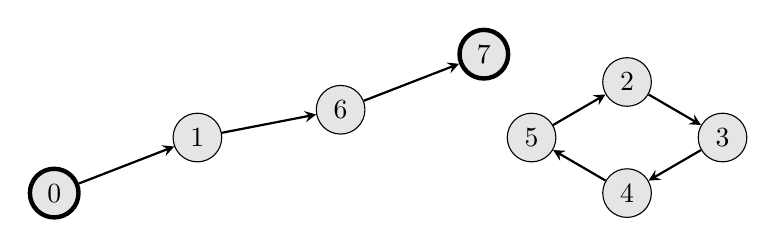
\begin{tikzpicture}[>=stealth, main/.style = {draw, circle, fill=black!10!white}]
		\centering

		\node[main, ultra thick] (0) at (0.1\textwidth,-20bp) {0};
		\node[main] (1) at (0.25\textwidth,0bp){1};
		\node[main] (6) at (0.4\textwidth,+10bp){6};
		\node[main, ultra thick] (7) at (0.55\textwidth,+30bp) {7};

		\node[main] (2) at (0.7\textwidth, +20bp){2};
		\node[main] (3) at (0.8\textwidth, -0bp) {3};
		\node[main] (4) at (0.7\textwidth, -20bp) {4};
		\node[main] (5) at (0.6\textwidth, -0bp) {5};

		\draw [->,thick] (0) -- (1);
		\draw [->,thick] (1) -- (6);
		\draw [->,thick] (6) -- (7);

		\draw [->,thick] (2) -- (3);
		\draw [->,thick] (3) -- (4);
		\draw [->,thick] (4) -- (5);
		\draw [->,thick] (5) -- (2);
	\end{tikzpicture}

	\centering
	\caption{
		An example of a path containing spurious unconnected subtours,
		over a network with $V^\prime = \Set*{0, \dots, 7},\ s = 0,\ t = 7$.
		The SEC inequalities of \cref{eq:espprc-sec-constraints} prohibit the depicted situation from occurring.
	}
	\label{fig:espprc-example-with-spurious-subtours}
\end{figure}

\begin{figure}[ht]
	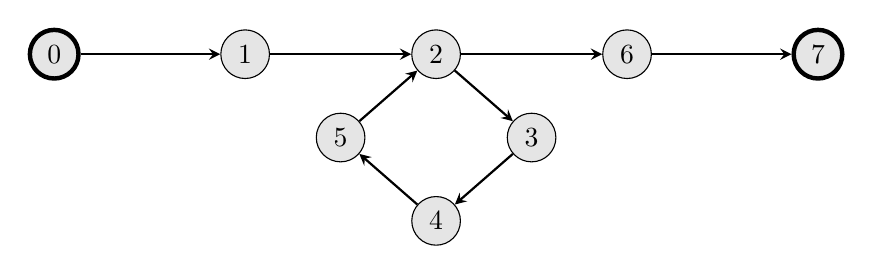
\begin{tikzpicture}[>=stealth, main/.style = {draw, circle, fill=black!10!white}]
		\centering

		\node[main, ultra thick] (0) at (0.1\textwidth,0bp) {0};
		\node[main] (1) at (0.3\textwidth,0bp){1};
		\node[main] (2) at (0.5\textwidth,0bp){2};
		\node[main] (3) at (0.6\textwidth,-30bp) {3};
		\node[main] (4) at (0.5\textwidth,-60bp) {4};
		\node[main] (5) at (0.4\textwidth,-30bp) {5};
		\node[main] (6) at (0.7\textwidth,0bp){6};
		\node[main, ultra thick] (7) at (0.9\textwidth,0bp) {7};

		\draw [->,thick] (0) -- (1);
		\draw [->,thick] (1) -- (2);
		\draw [->,thick] (2) -- (3);
		\draw [->,thick] (3) -- (4);
		\draw [->,thick] (4) -- (5);
		\draw [->,thick] (5) -- (2);
		\draw [->,thick] (2) -- (6);
		\draw [->,thick] (6) -- (7);
	\end{tikzpicture}

	\centering
	\caption{
		An example of a path not satisfying the elementarity constraints,
		over a network with $V^\prime = \Set*{0, \dots, 7},\ s = 0,\ t = 7$.
		The SEC inequalities of \cref{eq:espprc-sec-constraints} prohibit the depicted situation from occurring.
	}
	\label{fig:espprc-example-non-elementary-solution}
\end{figure}

As it is done in \textcite{beasley1989},
if one wishes to avoid the formation of spurious unconnected subtours
while relaxing the elementarity condition,
it can achieve so by substituting \cref{eq:espprc-sec-constraints} in favor
of a big-M constraint of the form:
\begin{equation}
	\label{eq:espprc-relaxed-elementarity}
	\ExprESPPEdgesWithin[S] \le M \ExprESPPEdgesCrossing[S] \quad \forall S \subseteq V_0 \cup \Set*{s},
\end{equation}
where $M \in \R_+$ denotes an arbitrary large positive constant.
\Cref{eq:espprc-relaxed-elementarity} avoids the situation depicted
in \cref{fig:espprc-example-with-spurious-subtours}
while permitting the situation depicted in \cref{fig:espprc-example-non-elementary-solution}.
Modeling the pricing as an SPPCC can significantly reduce column generation running time
but at the expense of significantly weaker dual-bound improvements.
For more information, refer to the discussion in \cref{sec:solving-the-pricing-problem}.

Valid inequalities and a branch-and-cut framework for the ESPPCC
are discussed in the work of \textcite{jepsen2008branchandcut}.
The CPTP in the context of pricing is the primary focus of this thesis.
As a result, we will not spend any more time discussing the ESPPCC.

\section{The Capacitated Profitable Tour Problem}
\label{sec:the-capacitated-profitable-tour-problem}

The \textit{Capacitated Profitable Tour Problem}, abbreviated as CPTP,
belongs to the group of the so-called
\textit{Travelling Salesman Problems with Profits} (TSPP) (see \cite{feillet2005})
and thus share many similarities with other studied optimization problems such as:
(i) the \textit{Orienteering Problem} (OP) \parencite{golden1987, laporte1990}
(ii) the \textit{Profitable Tour Problem} (PTP) \parencite{dellamico1995},
(iii) the \textit{Prize Collecting Traveling Salesman Problem} (PCTSP) \parencite{balas1989prize, balas1995prize},
(iv) the \textit{Capacitated m-Ring-Star Problem} (CmRSP) \parencite{baldacci2007capacitated}.
Refer to \textcite{letchford2013} for the Steiner extension of these problems.

The OP, an NP-hard problem \parencite{laporte1990}, asks for a route serving
a subset of customers with associated profits.
In the OP, the route length is limited by the number of vertices visited,
whereas, in CPTP,
the route length is constrained by the accumulated demand served.
We can conclude that CPTP is NP-hard by applying the same reasoning
to prove that the OP is NP-hard in \textcite{laporte1990}.
The OP is equivalent to an edge-capacitated CPTP with unit demands.
For contributions introducing BAC frameworks and valid inequalities for the OP,
see \textcite{fischetti1998, gendreau1998}.
Many of these inequalities (but not all) extend to the CPTP as shown in \textcite{jepsen2014}.

The CPTP is a special case of ESPPCC where the source and sink vertices coincide.
The CPTP, like the ESPPCC, can model the pricing sub-problem for the CVRP.
In contrast to the more general ESPPRC formulation, the CPTP is much easier to describe.
However, because of its narrower scope, it is a problem that receives far less attention in the literature.
To our knowledge, the few contributions to studying the CPTP in the context of pricing
for the CVRP are \textcite{jepsen2011,jepsen2014}.
not considering non-robust inequalities at the RMP level.

\medskip

In more detail,
the CPTP is a combinatorial optimization delivery problem,
in which,
given as input a fully connected undirected network where vertices represent the customers,
the goal resides in finding a resource-constrained elementary tour (or circuit)
starting from a common point called the depot,
that minimizes the overall travel distance while maximizing
the profits associated with serving only a subset of the customers.
Each customer's profit lowers the tour cost only if the corresponding node is visited.
Because of the elementarity constraint,
vertices cannot be visited multiple times,
implying that the earnable profit per customer is only available once.
The profit is encoded at the node level in the traditional CPTP formulation \parencite{jepsen2014}
rather than being included directly in the definition of the reduced cost variable
$\bar{c}_{ij} \quad \forall i, j \in V_0 \cup \Set*{0}$ as it is in the ESPPCC.

The presentation of this section, as well as the implementation discussed
in \cref{sec:implementation-chapter},
owes a lot to the original efforts of \textcite{jepsen2014}.

\subsection{Integer Programming formulation}
\label{sec:cptp-integer-programming-formulation}

We present a CPTP formulation that closely resembles the formulation provided in \textcite{jepsen2014}.
In terms of mathematical notation, we will use and extend the original
mathematical constructs introduced for the CVRP in \cref{sec:cvrp-mathematical-notation}.

Let $p_i \in \R$ denote the profit associated in visiting a vertex $i \in V$.
The profit function is directly related to the dual variables $\pi \in \R^N$ associated to
the RMP's constraints of \cref{eq:mp-K-routes,eq:mp-customers-visited-by-exactly-one-route}.
Namely, $p_i = \pi_i \quad \forall i \in V$.

Let $x_{e}$, $y_{i} \in \Set*{0, 1}$ be two sets of binary decision variables which respectively
model whether an undirected edge $e \in E$ or vertex $i \in V$ is covered by the optimal CPTP route.
We can provide a formal mathematical description of the CPTP through an Integer Program (IP) formulation:
\begin{align}
	\min_{x,y} \quad z_\mt{CPTP}(x, y) & = \ExprCptpObjValDef                     & \label{eq:cptp-obj-function}                                                                          \\
	                                   & y_0 = 1                                  & \label{eq:cptp-depot-part-of-tour-constraint}                                                         \\
	                                   & \ExprCptpDemandSum  \le Q                & \label{eq:cptp-resource-upper-bound-constraint}                                                       \\
	                                   & \ExprCptpEdgesIncident{i}  = 2 y_i       & \quad \forall i \in V         \label{eq:cptp-flow-conservation-constraint}                            \\
	                                   & \ExprCptpFlowExiting{S} \ge 2 y_{i}      & \quad \forall i \in S,\ \forall S \subseteq V_0,\ \SetSize*{S} \ge 2 \label{eq:cptp-gsec-constraints} \\
	                                   & x_{e}                   \in \Set*{0, 1}  & \quad \forall e \in E               \label{eq:cptp-x-mip-var-bounds}                                  \\
	                                   & y_{i}                    \in \Set*{0, 1} & \quad \forall i \in V             \label{eq:cptp-y-mip-var-bounds},
\end{align}
where \labelcref{eq:cptp-obj-function} is the objective function to be minimized, i.e. the cost
accounting for the total travel distance and the profit in serving a subset of the vertices.
Constraint \labelcref{eq:cptp-depot-part-of-tour-constraint} ensures that the depot is always covered by the optimal route.
Constraint \labelcref{eq:cptp-resource-upper-bound-constraint} is the resource consumption upper bound.
Constraint \labelcref{eq:cptp-flow-conservation-constraint} has a twofold effect.
First, it functions as a form of directed flow conservation.
Second, it links the $x,\ y$ sets of variables together;
namely, it ensures that the if a vertex $i \in V$ is covered by an optimal route ($y_i = 1$)
then the number of incident edges in that node sums to $2$, otherwise to $0$.
Constraint \labelcref{eq:cptp-gsec-constraints}
are the so-called Generalized Subtour Elimination Constraints (GSECs),
which avoid the formation of spurious tours in unconnected regions of the network.
Because there are an exponential number of GSECs,
these constraints cannot be inserted statically in a MIP solver
and must instead be separated exactly, at least for integral solutions.
Constraints \labelcref{eq:cptp-x-mip-var-bounds,eq:cptp-y-mip-var-bounds} respectively
impose bounds and integrality conditions
on the number of traversal for edges $e \in E$ and vertices $i \in V$.
The IP model consists of $\frac{N^2 + N}{2}$ number of binary variables and an exponential number of constraints.
If we ignore the GSECs and variable bounds, the IP model owns a total of $N + 2$ constraints.
Constraints \labelcref{eq:cptp-gsec-constraints}
can also be rewritten in a different form \parencite{wolsey2020integer}:
\begin{equation}
	\label{eq:cptp-gsec-constraints-v2}
	\sum\limits_{e \in E(S)} x_e \le \sum\limits_{i \in S \setminus \Set*{j}} y_i \quad \forall j \in S,\ \forall S \subseteq V_0,\ |S| \ge 2.
\end{equation}
Depending on the size of the subset $S \subseteq V_0, S \ge 2$,
\labelcref{eq:cptp-gsec-constraints-v2} may be sparser than \labelcref{eq:cptp-gsec-constraints}.
Equivalently, the constraint of \cref{eq:cptp-resource-upper-bound-constraint}
can be defined at the edge level:
\begin{equation}
	\label{eq:cptp-resource-upper-bound-constraint-edge-level}
	\sum_{e = \Set*{i, j} \in E} \frac{q_i + q_j}{2} x_e \le Q.
\end{equation}

Note that model
\labelcref{eq:cptp-obj-function,eq:cptp-depot-part-of-tour-constraint,eq:cptp-resource-upper-bound-constraint,eq:cptp-flow-conservation-constraint,eq:cptp-gsec-constraints,eq:cptp-x-mip-var-bounds,eq:cptp-y-mip-var-bounds}
does not permit for single-customer routes.
Instead of modifying the formulation to allow for this edge case,
it may be simpler to leave the model unchanged.
By employing a brute-force algorithm in $\Theta(N)$ time,
we scan for improving single-customer solutions.
After the resolution of the IP model,
we check for improving single-customer solutions and,
if any exist,
we update the incumbent as appropriate.

\subsection{Additional Valid Inequalities}
\label{sec:cptp-additional-valid-inequalities}

We present additional valid inequalities for the CPTP problem in this section.
While these additional inequalities are not strictly required
to ensure the correctness of the solution approach,
they can massively strengthen the linear relaxation
and thus speed up the resolution process when embedded within an efficient branch-and-cut framework.
However, devising efficient separation algorithms is critical to make such inequalities efficacious.

The inequalities presented here closely follow the presentation provided in \textcite{jepsen2014}.
For a complete list of CPTP valid inequalities compared to what we could give, see \textcite{jepsen2014}.
We will focus primarily on two valid inequalities in this thesis:
the \textit{Rounded Capacity Constraints} (RCC) discussed in \cref{sec:cptp-rcc}
and the \textit{Generalized Large Multistars} (GLM) discussed in \cref{sec:cptp-glm}.
We have focused solely on these two sets of inequalities for two reasons.
First, \textcite{jepsen2014} found that these two inequalities
are the most frequently separated,
implying that including them would likely speed up the resolution process.
Second, they can be reasonably separated utilizing
the same separation procedure employed for the GSEC inequalities.
See implementation details later in \cref{sec:impl-separation-techniques}.

\subsubsection{Rounded Capacity Constraints (RCC)}
\label{sec:cptp-rcc}

The \textit{Rounded Capacity Constraints}, or RCC for short,
were introduced for the CVRP in \textcite{laporte1983}
and were previously introduced in \cref{sec:cvrp-two-index-flow-formulation}.

Recall that $q(S) = \sum_{i \in S} q_i$ represents
the total demand in serving all vertices in set $S \subseteq V$.
The RCC constraints act as a capacity constraint
by requiring that any customer set $S \subseteq V_0$ be crossed by
a number of edges that is not less than the required trucks amount
to serve all customers in $S \subseteq V_0$.
\textcite{jepsen2014} extend the RCC inequalities to the CPTP:
\begin{equation}
	\label{eq:cptp-rcc-inequality-original}
	\ExprCptpFlowExiting{S} \ge 2 \ceil*{\frac{\sum\limits_{i \in S} q_i y_i}{Q}} \quad \forall S \subseteq V_0,\ |S| \ge 1.
\end{equation}
\Cref{eq:cptp-rcc-inequality-original} is very similar
to the CVRP's RCC of \cref{eq:two-index-flow-ccc-bpp-lb},
except that the right-hand side is composed of model's variables instead of constants.
Notice that such approach is correct since $\sum_{e \in \delta(S)} x_e \in \Z_+$.
Unfortunately, because the ceil function is a non-linear operation,
such a constraint cannot be reported to most MIP solvers.

Fortunately, \textcite{baldacci2007capacitated} provides a way to
combat this undesirable aspect at the cost of obtaining a looser bound of the RCC.
Namely, given $\alpha, \beta, \gamma \in Z_+$, with $\alpha > \gamma$ and
$\fmod{\alpha}{\gamma} \ne 0$, the following result holds:
\begin{equation}
	\label{eq:baldacci-rcc-theorem-weaker-bound}
	\ceil*{\frac{\alpha - \beta}{\gamma}} \ge \ceil*{\frac{\alpha}{\gamma}} - \frac{\beta}{\fmod{\alpha}{\gamma}}.
\end{equation}
\textcite{jepsen2014} claim that \cref{eq:baldacci-rcc-theorem-weaker-bound}
holds even when $\alpha > \gamma$ is not satisfied
(unfortunately the authors don't provide further explanations on why this is the case).

By picking $\alpha = q(S) = \sum_{i \in S} q_i,\ \beta = \sum_{i \in S} q_i\Expr*{1 - y_i},\ \gamma = Q$,
we obtain the following linear, but weaker, RCC:
\begin{equation}
	\label{eq:cptp-rcc-inequality}
	\sum\limits_{e \in \delta(S)} x_e \ge 2 \Expr*{\ceil*{\frac{q(S)}{Q}} - \frac{\sum\limits_{i \in S} q_i \Expr*{1 - y_i}}{\ExprQr(S)}} \quad \forall S \subseteq V_0,\ |S| \ge 1,
\end{equation}
where $\ExprQr(S) = \fmod{q(S)}{Q}$ is the remainder capacity associated
to an arbitrary set $S \subseteq V$.
Notice, that \cref{eq:baldacci-rcc-theorem-weaker-bound} guarantees correctness
of the \cref{eq:cptp-rcc-inequality} only if $q_i \in Z_+ \quad \forall i \in V_0$ holds.
Fortunately, this is true for the vast majority of the routing problems considered in the literature.

As \textcite{jepsen2014} points out,
no exact separation procedure is currently known for the RCC inequalities,
for this reason,
they suggest using the characterizing sets identified by the separation of the multistar inequalities,
such as the GLM separation procedure.
See the next \cref{sec:cptp-glm}.

\subsubsection{Generalized Large Multistar (GLM)}
\label{sec:cptp-glm}

The \textit{Generalized Large Multistar} inequalities,
or GLMs for short,
were first proposed in \textcite{gouveia1995} for the CVRP.
The GLMs were further generalized
to the so-called \textit{Knapsack Large Multistar} (KLM) inequalities in \textcite{letchford2002}.
\textcite{letchford2006} investigates the effectiveness of the multistar family of cuts
when applied to vehicle routing problems.
The multistar cuts are a collection of inequalities
related to the intersection  of the 0--1 knapsack and the CPTP polytopes.

Consider the capacity inequality:
\begin{equation}
	\label{eq:cptp-weaker-rcc}
	\sum_{e \in \delta(S)} x_e \ge \frac{2}{Q} \sum_{i \in S} d_i y_i \quad \forall S \subseteq V_0,\ |S| \ge 2,
\end{equation}
which is a weaker version of the RCC in \cref{eq:cptp-rcc-inequality-original},
where the ceiling is not applied.
\Cref{eq:cptp-weaker-rcc} can be improved to obtain the GLM inequalities
by noting that nodes $j \notin S$ are also visited when the crossing edges $\delta(S)$ are used.

The GLM inequalities can be expressed as \parencite{jepsen2014}:
\begin{equation}
	\label{eq:cptp-glm-inequality}
	\sum\limits_{e \in \delta(S)} x_e \ge \frac{2}{Q} \Expr*{
		\sum\limits_{i \in S} q_i y_i +
		\sum\limits_{\EqStackTwo{e = \Set*{i, j} \in \delta(S)}{i \in S,\ j \notin S}} q_j x_e
	}
	\quad \forall S \subseteq V_0,\ |S| \ge 2.
\end{equation}

The general idea behind multistar inequalities is the following.
The vehicle must have sufficient capacity to serve
all of the customers covered by $S$
and all other customers outside $S$
who are connected to nodes in $S$ through a crossing edge $e = \Set*{i, j},\ i \in S,\ j \notin S$.
The "capacity" in GLM is measured in terms of the number of vehicles,
which is found by dividing by $Q$ the corresponding demand.
GLM inequalities are efficiently separable with
an exact polynomial-time procedure by finding minimum
$(u, v)$-cuts $\forall u \in V_0,\ v = 0$
in a directed flow network with capacities that depend on the vertex $u$
\parencite{letchford2006, jepsen2014}.
A simpler approach is to use a heuristic approach
by minimizing only the term $\sum_{e \in \delta(S)} x_e$ as to stress the violation.
This can be achieved by computing $(u, v)$-cuts $\forall u \in V_0,\ v = 0$
in a directed flow network where capacities are given exclusively from the
fractional solution $x^\star_{\Set*{i, j}} \quad \forall i, j \in V$.
See implementation details later in \cref{sec:impl-separation-techniques}.
